% ═══════════════════════════════════════════════════════════════════════════════
\section{Special Economic Zone Effectiveness}
\label{sec:sez}
% ═══════════════════════════════════════════════════════════════════════════════

\subsection{The Theoretical Role of SEZs in GVC Embedding}

Special economic zones represent the spatial instrument through which developing country governments attempt to create investment-grade institutional conditions within a constrained geographic perimeter, bypassing the slower and politically more difficult process of national-level reform. The logic is straightforward: if regulatory quality, customs efficiency, and infrastructure are inadequate at the national level to attract export-oriented FDI, create a bounded territory where those conditions do prevail, and use it as both an immediate FDI attractor and as a demonstration project that can generate political support for broader reforms \citep{farole2011}.

The literature on SEZ effectiveness is, however, sharply divided. Wang (2013) finds large positive effects of Chinese SEZs on manufacturing output and FDI in treated regions. Farole (2011), analysing SEZs across Africa and South Asia for the IFC, finds that fewer than one-third of SEZs in developing countries achieve their FDI attraction targets, primarily due to inadequate infrastructure investment, overly restrictive land allocation processes, and failure to develop backward linkages with the domestic economy. The critical distinction, as Zeng (2016) identifies, is between ``standalone'' SEZs --- isolated industrial estates with no backward linkage policy --- and ``networked'' SEZs that are integrated into national education, supplier development, and logistics systems. Vietnam's export processing zones (EPZs) are widely cited as exemplary of the networked model; several of Uzbekistan's zones more closely resemble the standalone model.

\subsection{Uzbekistan's SEZ Landscape}

As of 2023, Uzbekistan operates 21 free economic zones (FEZs) and over 100 small industrial zones and technology parks at the regional level, making it one of the most SEZ-intensive economies in the post-Soviet space by zone count per capita. Table~\ref{tab:sez_overview} summarises the principal zones with national significance.

\begin{table}[H]
 \centering
 \caption{Principal Special Economic Zones in Uzbekistan: Overview}
 \label{tab:sez_overview}
 \small
 \begin{tabular}{@{}p{2.8cm}p{1.3cm}p{2.5cm}p{1.5cm}p{2.8cm}@{}}
 \toprule
 SEZ & Est. & Primary Sector & FDI Attracted (cum. USD m) & Northeast Asian Anchor \\
 \midrule
 Navoiy FIEZ & 2008 & Aviation logistics, textiles & \$580 & Korean Air Cargo (logist.) \\
 Jizzakh FEZ & 2013 & Electronics, light mfg. & \$320 & Artel (Samsung tech) \\
 Urgench FEZ & 2013 & Textiles, food processing & \$140 & --- \\
 Sirdaryo FEZ & 2013 & Chemical products & \$90 & --- \\
 Angren FEZ & 2012 & Metals, construction mat. & \$210 & Peng Cheng Park (CHN) \\
 Tashkent IT Park & 2019 & ICT services & \$45 & Samsung, Huawei (tech transfer) \\
 Termez Logistics & 2021 & Transit logistics & \$30 & --- \\
 Khorezm FEZ & 2022 & Textiles, ceramics & \$20 & --- \\
 \bottomrule
 \end{tabular}
 \\\smallskip
 \small FDI attracted: cumulative investment received from inception through 2023. Source: Uzinfoinvest; Uzbek Ministry of Investments and Foreign Trade; author collation.
\end{table}

The landscape reveals several features relevant to GVC embedding. First, the cumulative FDI attracted across all major FEZs totals approximately \$1.4 billion --- a figure that is modest relative to the scale needed for transformative industrialisation (Vietnam's single Binh Duong Province attracted over \$30 billion FDI in its first 20 years of operation). Second, Northeast Asian anchor investments are present but thin: Korean Air's cargo hub at Navoiy, Artel's (Samsung-technology-licensed) electronics assembly at Jizzakh, and China's Peng Cheng industrial park at Angren represent the principal GVC-relevant investments. Third, the zones are geographically dispersed across Uzbekistan's regions without clear spatial concentration --- a pattern that diffuses infrastructure investment across multiple locations rather than creating a single high-quality industrial cluster.

\subsection{SEZ Incentive Structure}

Uzbekistan's FEZ incentive packages include: (i) ten-year corporate income tax exemption; (ii) exemption from land tax and property tax for the exemption period; (iii) VAT exemption on imported capital goods and raw materials; (iv) 50\% reduction in personal income tax for foreign workers; and (v) streamlined single-window customs procedures within zone boundaries.

This incentive structure is broadly competitive with Vietnamese EPZ incentives at the comparable stage. Table~\ref{tab:sez_incentives} provides a direct comparison.

\begin{table}[H]
 \centering
 \caption{SEZ Incentive Comparison: Uzbekistan FEZ versus Vietnam EPZ versus Thailand BOI Zone}
 \label{tab:sez_incentives}
 \small
 \begin{tabular}{@{}lccc@{}}
 \toprule
 Incentive Dimension & Uzbekistan FEZ & Vietnam EPZ & Thailand BOI Zone A \\
 \midrule
 Corporate tax holiday (years) & 10 & 4 (renewable) & 8 \\
 Import duty on capital goods & 0\% & 0\% & 0\% \\
 Import duty on raw materials & 0\% & 0\% & 0\% \\
 Export duty & 0\% & 0\% & 0\% \\
 Land lease rate (USD/m$^2$/year) & \$1.0 & \$2.5--\$4.0 & \$3.0--\$5.0 \\
 One-stop shop & Partial & Full & Full \\
 Infrastructure quality (index 0--5) & 3.1 & 3.8 & 4.2 \\
 \bottomrule
 \end{tabular}
 \\\smallskip
 \small Infrastructure quality index: author assessment based on World Bank Enterprise Surveys and ADB infrastructure assessments. Source: UNCTAD Investment Policy Monitor; Vietnam EPZ/IZ Law; Thailand BOI Promotion Criteria 2023.
\end{table}

The incentive packages are not the binding constraint: Uzbekistan's tax holidays are longer and land costs lower than Vietnam's and Thailand's. The critical deficits are in one-stop-shop completeness and infrastructure quality. Investors consistently report that the ``single window'' in most Uzbek FEZs remains fragmented across multiple agencies, with customs, sanitary inspection, and fire safety approvals requiring separate applications to separate authorities. Vietnam's full single-window system, established through Decree 23/2007, consolidates all approvals into a single agency interface; Uzbekistan's Presidential Decree No.~5564 (2019) mandated equivalent consolidation but implementation has been uneven.

\subsection{The Navoiy Model: Aviation Logistics as a Landlocked GVC Solution}

Navoiy FIEZ represents Uzbekistan's most successful SEZ by international standards and deserves detailed attention because it represents a GVC integration model specifically tailored to landlocked geography. Rather than competing with coastal economies on maritime freight logistics, Navoiy has positioned itself as a transcontinental air cargo hub, leveraging its geographic position near the centre of the Eurasian landmass and its existing airport infrastructure (originally constructed for Soviet aviation).

Korean Air Cargo operates a hub-and-spoke air cargo service from Navoiy, connecting Northeast Asia (Incheon, Narita) to European destinations via Navoiy as an intermediate hub. This arrangement provides Uzbekistan with a GVC-relevant service: it enables high-value, time-sensitive goods (electronics components, pharmaceutical intermediates, automotive electronics) to transit through Uzbekistan, with the potential for value-adding processing within the FEZ before re-export. Garment manufacturers in Navoiy can use Korean Air Cargo to receive fabric from South Korea and ship finished garments to European buyers within 24--48 hours, a transit time that is not achievable by rail or road through Central Asian corridors.

The Navoiy model is not directly replicable across the entire economy: air freight costs limit its applicability to high-value-to-weight ratios. But it demonstrates that landlocked geography is not a universal constraint --- for specific product categories, air connectivity can substitute for maritime access and enable GVC integration that surface transit cannot. This insight should inform the product-sector targeting of Uzbekistan's SEZ promotion strategy.

\subsection{SEZ Performance Assessment: A Comparative Scorecard}

Figure~\ref{fig:sez_performance} presents a comparative assessment of SEZ performance across the key effectiveness dimensions identified by \citet{farole2011}: FDI intensity, export performance, employment generation, backward linkage development, and technology transfer.

\begin{figure}[H]
 \centering
 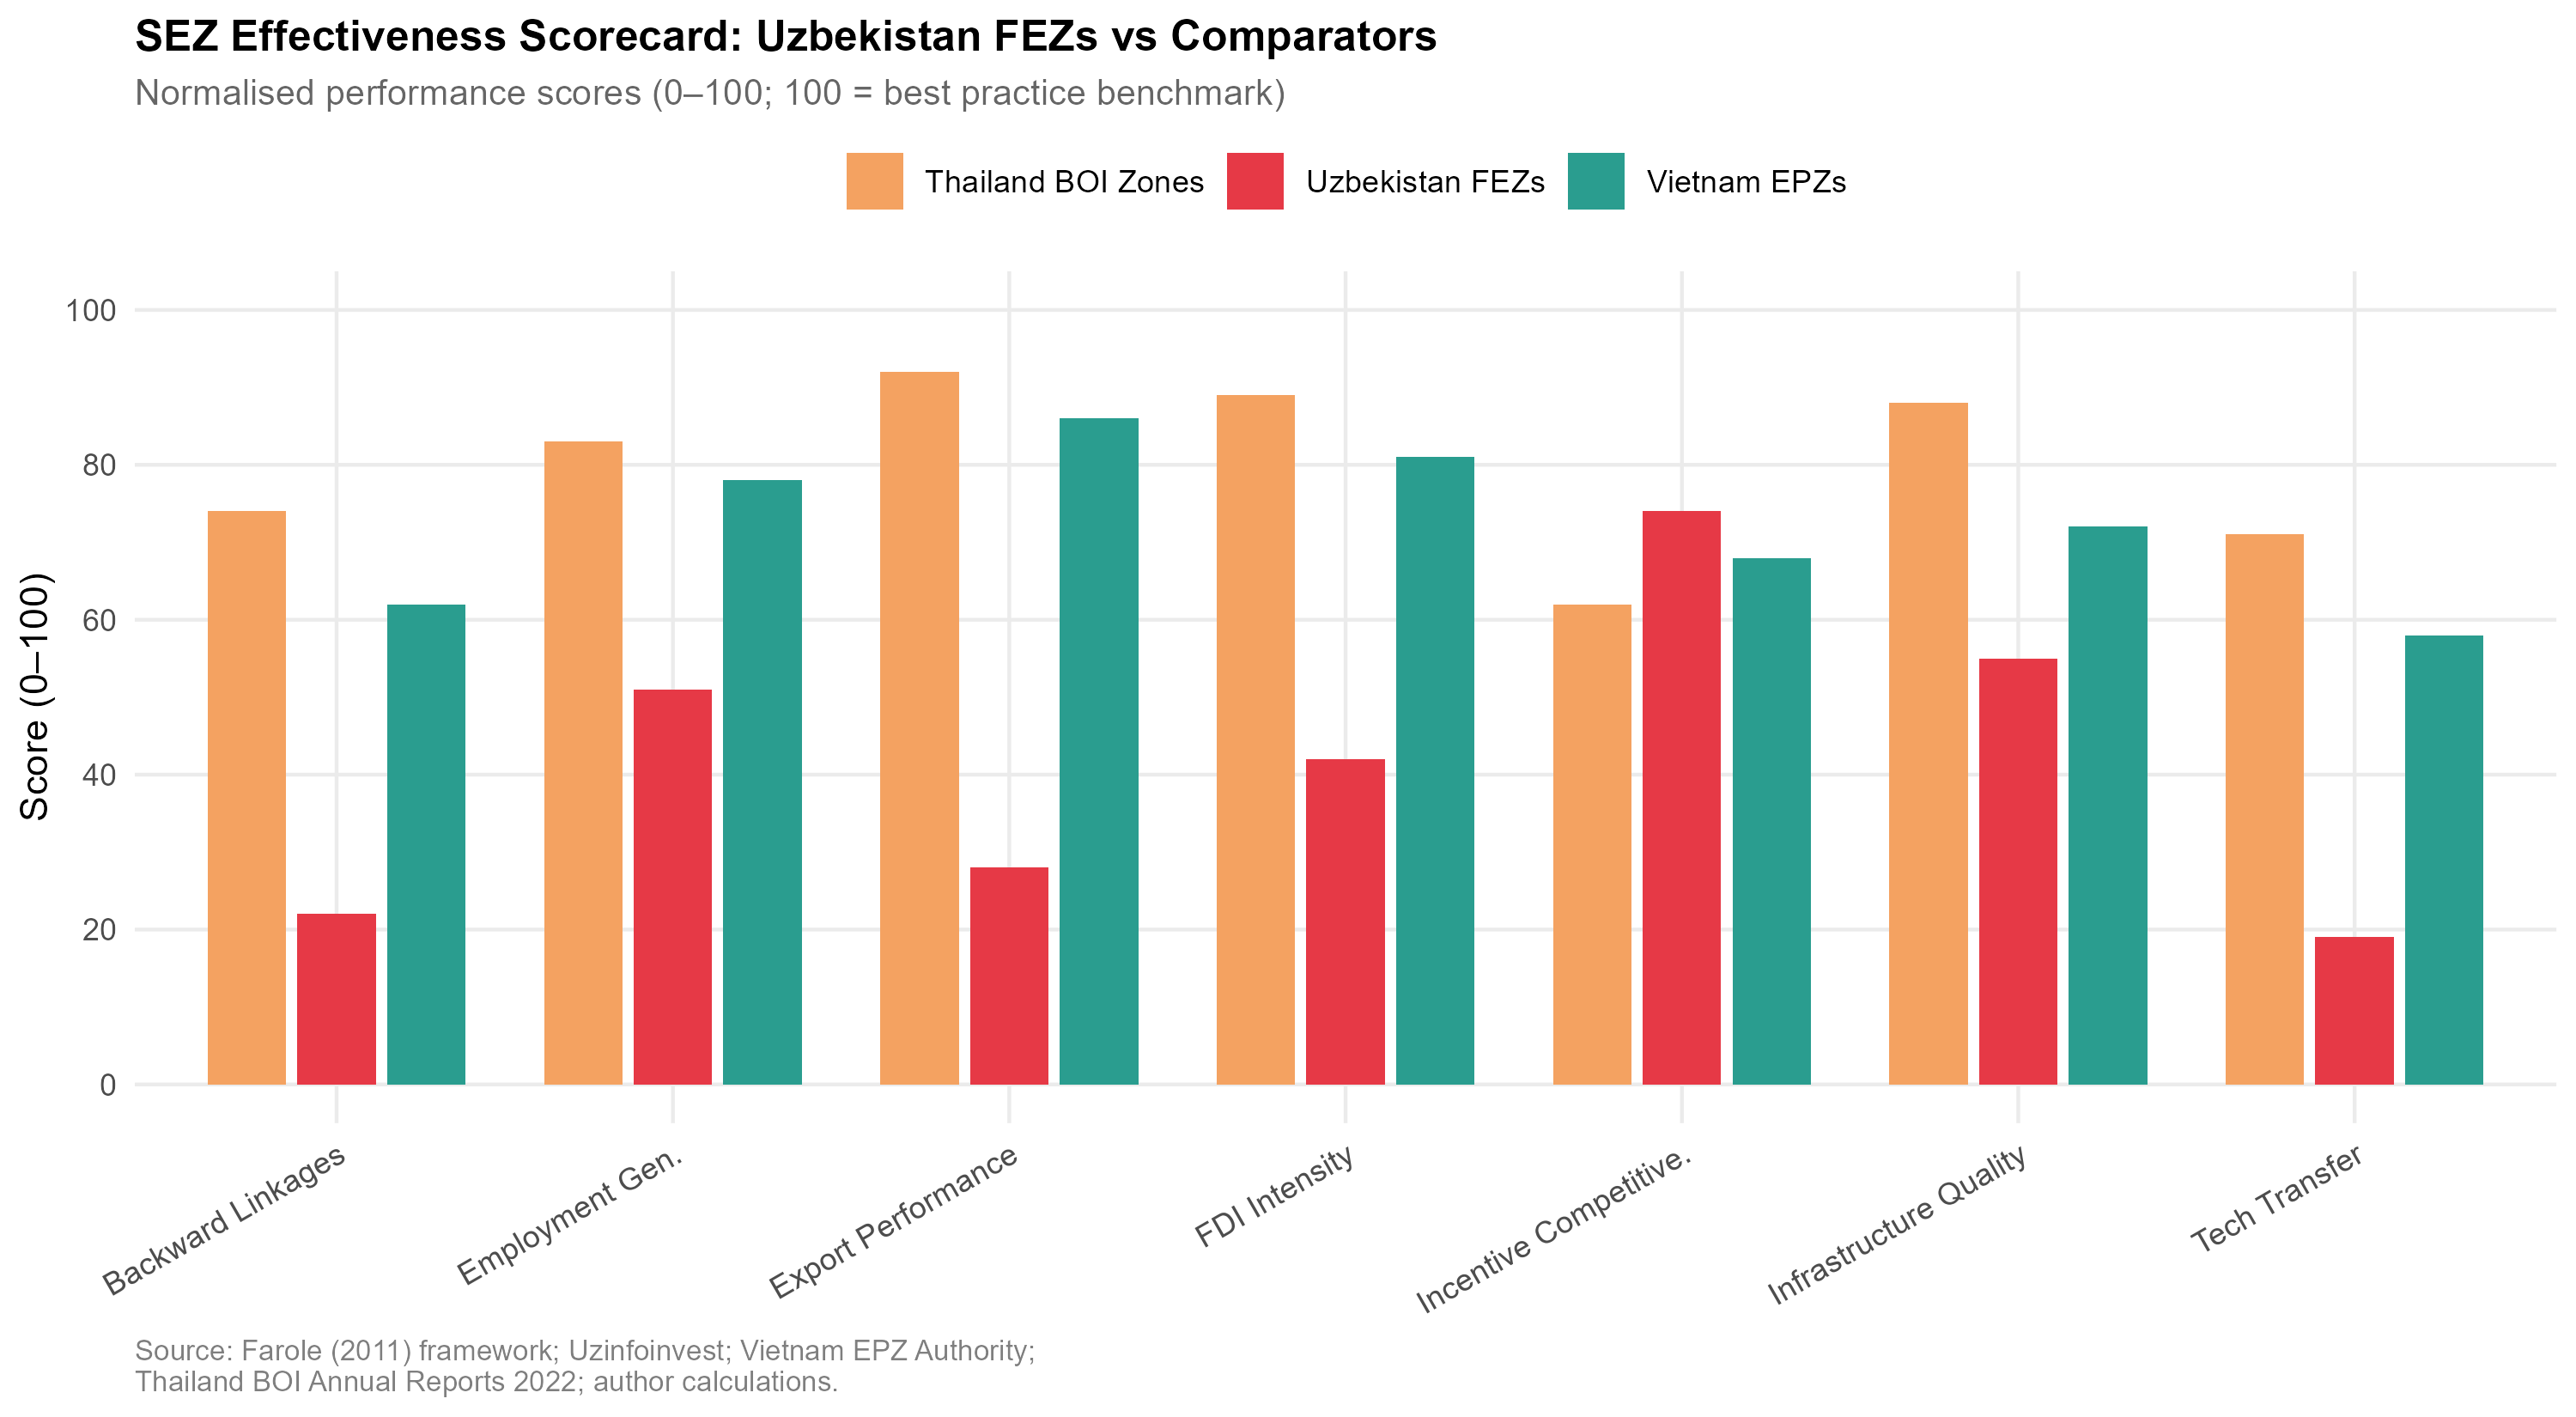
\includegraphics[width=0.90\textwidth]{figures/fig20_sez_performance.png}
 \caption{SEZ Effectiveness Scorecard: Uzbekistan FEZs vs.\ Vietnam EPZs and Thailand BOI Zones. Bars represent normalised performance scores (0--100, where 100 = best practice benchmark). Source: Farole (2011) framework; Uzinfoinvest; Vietnam EPZ Authority; Thailand BOI Annual Reports; author calculations.}
 \label{fig:sez_performance}
\end{figure}

The assessment reveals that Uzbekistan's FEZs perform near or above comparator benchmarks on fiscal incentive competitiveness and land cost attractiveness, confirming that the policy design is appropriate. The underperformance is concentrated in export performance, backward linkage development, and technology transfer --- the outcomes most critical for GVC embedding rather than simple FDI attraction.

This pattern is consistent with Farole's (2011) characterisation of ``stunted'' SEZs: zones that succeed in attracting initial investment (and thus appear successful by FDI headline metrics) but fail to generate the multiplier effects --- domestic supply chain development, knowledge spillovers, worker skill upgrading --- that make SEZs engines of broader structural transformation. The policy implication is that Uzbekistan's SEZ strategy needs to shift from incentive competition to ecosystem development: building the supplier networks, training institutions, and logistics connectors that would make existing zone investments deepen and expand.
